\chapter{Nonlinear Forward model}
\begin{itemize}
	\item updating scheme, slow
	\item local linear map, strategy, schematic
	\item affine function, RTO
\end{itemize}

\section{Sampling}

\begin{figure}[h]
	\centering
	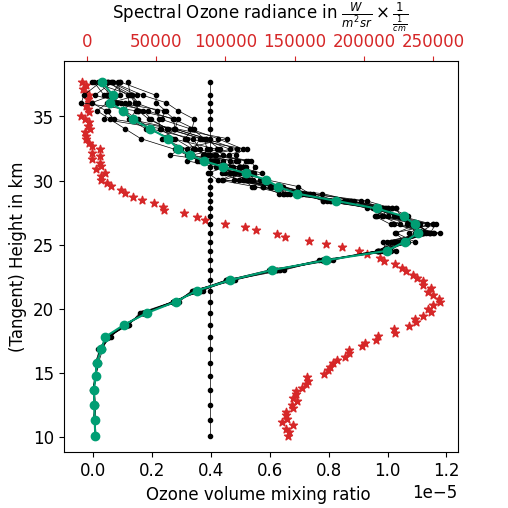
\includegraphics[width=\textwidth]{NonLinFirstRecRes.png}
	\caption[]{text}
	\label{fig:Results}
\end{figure}

\section{local linear Map and strategy}
\begin{itemize}
	\item one data vector
	\item strategy to find convergence and local linear map
\end{itemize}
\subsection{Machine learning vs Gaussian elimination}
\begin{itemize}
	\item linear solve
	\item machine learning class optimizer which package
\end{itemize}
\section{affine RTO}
\begin{itemize}
	\item does it sample from the correct distribution
\end{itemize}